\documentclass[../main.tex]{subfiles}
\begin{document}

\chapter{Introduction}
\labch{intro}

\section{The old nature-nurture debate}

Both genes and environment play a crucial role during the entire life of 
an organism, from development to senility, and in particular in the 
manifestation of complex diseases. Every phenotype arises as a 
consequence of the interactions of genes both with each other and with 
the environment. Other things being equal, genetic variation among 
individuals\cite{1000GenomesProjectConsortium2015} results in phenotypic 
variation; on the other hand, environment can influence a trait as much 
as any gene, especially if the trait is \textit{complex}.

A complex trait, as opposed to a mendelian trait, is a phenotype whose 
variation in the population cannot be explained by the variation in a 
single gene. For instance, height is a complex trait as there have been 
found many loci contributing to it: each of them gives a small 
contribution, and the final height depends on the combination of all the 
alleles in the individual's genome. Clearly, not \textit{all} phenotypic 
variation in a population can be explained by genetic variation, for the 
environment has an effect as well. The proportion of phenotipic variance 
that can be explained by genetic variance is called heritability (see 
\refsec{heritability}), which for height is about 
80\%\cite{Visscher2008a}. It cannot be said that an allele determines a 
phenotype, but rather variation at that locus can result in phenotypic 
variation (for instance disease status), under the influence of an 
appropriate environment.

One of the driving ideas of the Human Genome 
Project\cite{Lander2001,Venter2001} was that the knowledge of the human 
genome sequence and its annotation would have helped to explain and cure 
diseases. Indeed, epigenetic markers aside, DNA is the only heritable 
molecule, therefore heritable traits must be related to it. In 2005, a 
powerful method was developed in order to harness the huge amount of 
data collected from the sequencing of genomes: genome-wide association 
studies (see \refsec{gwas} for a technical description of the method), 
which find association between genetic variants and phenotypic traits, 
in the sense that people harbouring a particular allele might be more 
liable to develop a particular phenotype, and such liability can be 
quantified by an odds ratio (or effect size).

Gradually, it happened that the focus moved from candidate genes to 
whole genomes. As a consequence of the large amount of genetic variation 
among individuals, larger sample sizes were needed to study variation at 
a population level, thus many laboratories decided to join their forces 
to create consortia.

Another method to investigate complex traits is the mapping of loci that 
influence gene expression (see \refsec{eqtl}). Indeed, gene expression 
is an intermediate phenotype in the sense that it is one of the 
mechanistic steps that bring from a gene to an accomplished phenotype, 
therefore expression can be used as a proxy for the phenotype. In eQTL 
mapping, each SNP is assigned a coefficient according to how much the 
expression of a gene is altered by the presence of that SNP.

Environment can influence gene expression, and in fact also genes ---for 
instance, exposure to UV rays can cause mutations. However, since the 
effects of environment are difficult to quantify, much of the reaserch 
on complex traits and diseases was concerned on genetic factors. Here, 
our focus will be primarily on SNPs as genetic variants, and on humans 
as organisms of interest, with particular reference to their diseases.

\section{Genome-wide association studies and expression quantitative 
	trait loci mapping}

\marginnote{As of 2018-06-25, the GWAS Catalog contains 3420 
	publications and 62652 unique SNP-trait associations. 
	\url{https://www.ebi.ac.uk/gwas/home}}

The classical method to find associations between SNP and disease is the 
GWAS: several individuals in a cohort of cases and controls are 
genotyped, and the variants that occur more frequently in cases than in 
controls are said to be associated with the disease. Unless the full 
genome of the samples is sequenced, however, not every single variant in 
the population will be known, and in fact those that result associated 
to the disease are almost never the causal ones, but are only in linkage 
disequilibrium with the unknown causal SNP\cite{Visscher2012}. Moreover, 
even if the causal variant were known, we still would not know much 
about the mechanism or the underlying biology of the disease, although 
it is possible to leverage a functional annotation of the genome to draw 
conclusions\sidenote{For instance, most disease-associated SNPs fall in 
	enhancers, as reported in a paper by Ernst published in 2011, using 
	data from the ENCODE project.}.

Despite these limitations, GWAS have revealed some interesting facts. 
First and foremost, complex traits are highly 
polygenic\cite{Visscher2017}: there are many loci which, together, can 
carry a number of combination of alleles, each of which increases or 
decreases the probability of disease by a small amount. One of the 
hypothesis was that of \enquote{common disease, common variant}, but 
actually there can be few rare variants that contribute substantially to 
the disease risk, as well as many common variants with a small effect 
size. For some examples of success stories, see 
\reffig{introduction/gwas_success}.

\begin{figure}
	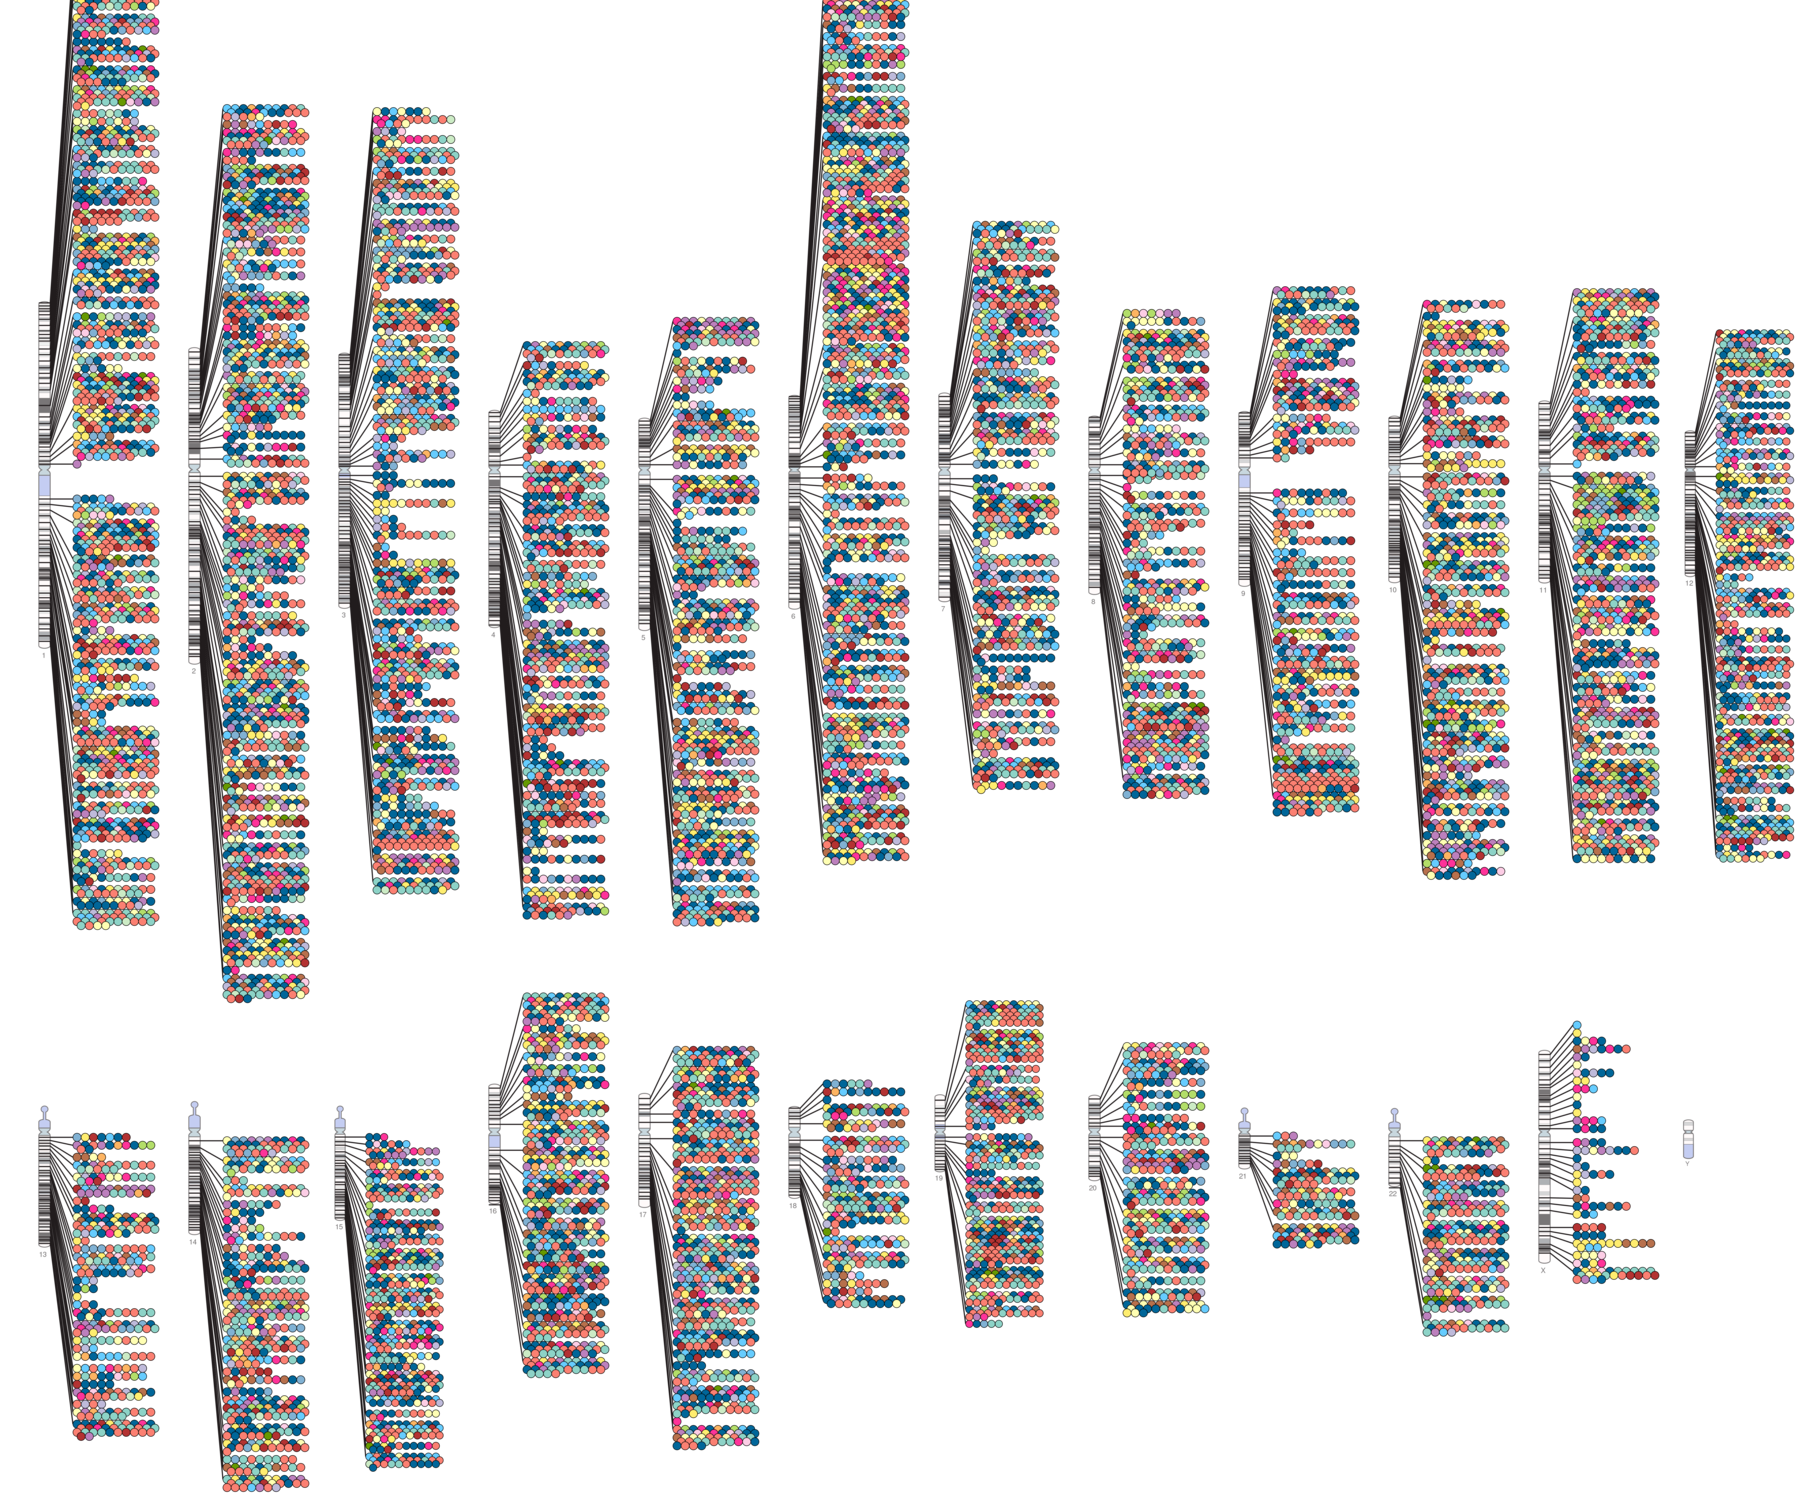
\includegraphics{introduction/gwas_success}
	\caption{Some success stories. For example, one of the genes 
		harbouring schizophrenia-associated variants is \textit{DRD2}, a 
		dopamine receptor; once the gene was known, drugs could be 
		developed.}
	\label{introduction/gwas_success}
\end{figure}

eQTL have resulted... many GWAS are eQTL

\section{Limits of GWAS and eQTL mapping}

Missing heritability.

%https://www.nature.com/articles/ng0508-489

%Combination of alleles may have specific effects both if they occur at 
%the same locus (dominance) or at different loci (epistasis). 

%\enquote{The main conclusion emerging from the current studies is that 
%GWAS are able to robustly identify common variants that are associated 
%with height but that the effect sizes of individual variants are small, 
%so that very large sample sizes are needed to detect associations 
%reliably. Single laboratories are unlikely to have sufficient sample 
%sizes to do powerful studies on their own, and the trend in human 
%complex trait mapping has been to create consortia of research groups 
%and even consortia of consortia.}

%At the same time, among the full sequences now available there are so 
%many variants that trying to associate them with anything is very 
%difficult. Statistics is not enough in this case.

%----

%other limit of gwas: they study single variants, but sometimes the 
%disease manifest only when there is a certain \textit{combination} of 
%variants.

%gamazon2015: Gwas on their own are not enough (cite 
%https://www.nature.com/articles/nature08494). in particular, there is a 
%missing link between the variant and the disease: how (not why, 
%\textit{how}) does the variant make one individual more susceptible to 
%a disease? It is not true that the nearest gene is always involved.

%gamazon2015: Many SNPs are found in regulatory regions, as evinced by 
%the fact that they overlap with DNaseI sites (is this true? read Gusev, 
%A. et al. Regulatory variants explain much more heritability than 
%coding variants across 11 common diseases. bioRxiv 004309 (21 April 
%2014).), and that they often are found in eQTL (see Nicolae, D.L. et 
%     al. 
%Trait-associated SNPs are more likely to be eQTLs: annotation to 
%enhance discovery from GWAS. PLoS Genet. 6, e1000888 (2010).)

\end{document}
